% This is samplepaper.tex, a sample chapter demonstrating the
% LLNCS macro package for Springer Computer Science proceedings;
% Version 2.20 of 2017/10/04
%
\documentclass{llncs}
%
\usepackage{graphicx}

\begin{document}
% Adicionado para por apenas os numeros sem headers
\pagestyle{myheadings}
\title{Development of text-mining solutions to facilitate lipid metabolism interpretation in Genome-Scale Metabolic Models}

\author{Adriano Silva\inst{1}\and
João Ribeiro\inst{1}\and
Emanuel Cunha\inst{1}}

\institute{University of Minho}
%
\maketitle              % typeset the header of the contribution
%
\begin{abstract}
Systems Biology is gaining importance in the unveil of cellular secrets. More precisely GSM models allow the contextualization of omic data and the progress of genomic engineering.
Still, the lack of macromolecule structural defined representation, such as lipids, is glaring.

-- Generic and defined duality

-- Resolution

\keywords{Genome-Scale Metabolic Models  \and Lipids representation.}
\end{abstract}
%
%
%
\section{Introduction}
\subsection{Context and motivation}
In the past two decades, Systems Biology has emerged as a discipline capable of integrating molecular biological knowledge into an understanding at a system level, from a complete, precise, and efficient perspective.
Biological systems are complex and oftentimes present non-linear relationships between their components. Accordingly, there is the need to understand and contextualize them.
Genome-scale metabolic models (GSM) are useful tools that integrate genomic, biochemical, and physiological knowledge for the better understanding of living organisms metabolism \cite{Zou2018,Tavassoly2018}. 
These approaches can guide strain optimization and the production of a compound with industrial interest, such as lipidic biofuel produced by optimized yeasts and microalgae \cite{Sawangkeaw2013}.

The reconstruction of GSM models is gaining importance, mainly impulsed by the advances and cost-effectiveness in technologies that led to high-throughput biological data.
Over 6000 GSM models were reconstructed in total \cite{Gu2019} since the reconstruction of the first GSM model in 1999 \cite{Edwards1999}.
Nonetheless, the pace of reconstruction of GSM models cannot keep up with the advancements of high-throughput technologies and thus \textit{omics} data. The lack of integration of new data into GSM models is a problem inherent to this growth discrepancy.

Besides the usefulness of these models, their reconstruction is limited due to the lack of biochemical and incorporated structural data.
More precisely, complex macromolecules are often represented in their generic version not giving any biochemical and structural information \cite{Gu2019}.
Particularly in the case of lipids, only a small number of reconstructed GSM models have structurally defined lipids with no or few relevant cross-references. 

The integration of molecular information can be done by taking advantage of the  \emph{de facto} databases such as SWISS LIPIDS \cite{Aimo2015} and  LIPID MAPS \cite{Sud2007}.
Molecular information is important to the reliably integrate and annotate models' information regarding the different structurally defined lipids.
A tool capable of annotating and linking the different lipid species represented in GSM models with relevant databases could improve models' interpretability. Such improvement could leverage the yield optimisation of lipidic biofuels {Sawangkeaw2013}.




\subsection{Objective}

The main objective of this project is to integrate synonyms and abbreviations of lipids from SWISS LIPIDS and LIPID MAPS into a graph-based database. Then, those synonyms and abbreviations will be used to link lipids present in GSM models and their molecular structures.

\section{State of art}
\subsection{Genome Scale Metabolic Models}
GSM models are computational tools that conjugate biochemical and genomic data from an organism, with the capacity to perform \emph{in silico} predictions of a given organism phenotype in specific environmental and genetic conditions \cite{Rocha2007,Zhou2021}.

Thus, these models are key to the contextualization of high-throughput data and helpful in many other applications such as metabolic engineering, production of biochemicals and bio-materials, prediction of enzyme functions, or even in the discovery of drug targets \cite{Gu2019,Kim2017}.
Therefore, it is important to integrate reliable biochemical data into the reconstruction of these models to ensure their accuracy and further interpretability \cite{Moseley2021,Passi2021}. 


\subsection{Lipid computational representation}
Lipids are macromolecules grouped into different classes according with their structural composition. 
They are composed by two biochemical different components, the head usually composed by polar groups and the tail composed by apolar carbon linked chains.  
The differences in lipid structural polarity conferes amphipathic characteristic to this macromolecule \cite{Fahy2011}. 
This means that in an hidrophilic environment the polar part of the molecule is atracted and the apolar one repelled.
This allows the generation of micelles, which is important for their biological roles such as being the principal cell membrane components, energy storage, and signaling molecules.

As represented in Fig.\ref{fig1}, lipid structures can be split into two different parts: the backbone and the side chains. The former is not variable for the whole class, remaining the same to the whole structurally defined lipids in the same class.
As for the side chains, their structure can vary in the same class in the number of double bonds, stereochemistry and length.

According to Fahy and collaborators \cite{Fahy2009}, lipids can be divided into eight main classes:Fatty acyls,Glycerolipids,Glycerophospholipids,Sphingolipids,Sterol Lipids,Prenol Lipids,Saccharolipids,Polyketides. 
Due to the myriad of side chain combinations, it is not possible to estimate how many distinct lipids can occur, both naturally and synthetically \cite{Gyamfi2018}.

\begin{figure}
    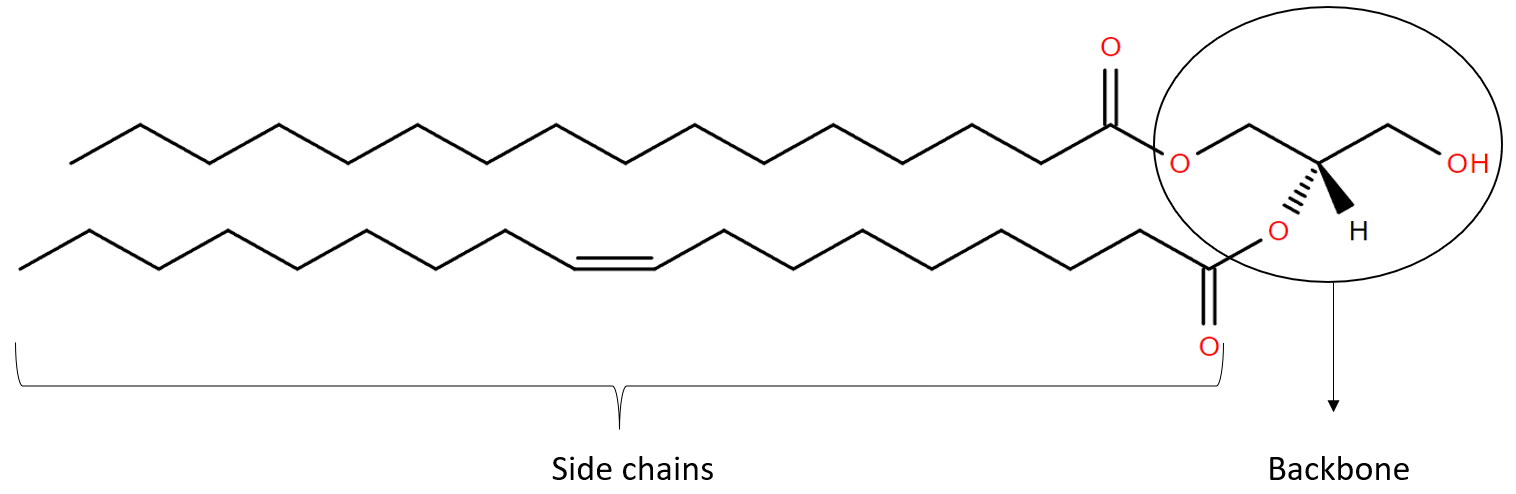
\includegraphics[width=\textwidth]{imagens/lipido.png}
    \caption{Representation of 1-hexadecanoyl-2-(9Z-octadecenoyl)-sn-glycerol structure extracted from LIPID MAPS. The backbone is the hydrophilic part of the lipid while the side chains confer hydrophobicity.} \label{fig1}
\end{figure}

The growing importance of this macromolecule in health research and industrial applications bring the need to characterize their metabolic network and roles in cells.
Due to the immense amount of reactions, complex lipid biosynthetic pathways, and their inherent combinatorial complexity, it is almost impossible to study them by means of classical molecular biology \cite{Schutzhold}.

Computational approaches and, particularly, GSM models are helping to disentangle these issues \cite{Schutzhold}, however, lipid representation in such models is not as trivial as desirable.
Despite the existence of lipid databases with defined structures, GSM models still fail to represent lipids with their structure completely defined \cite{Aung2013}. Nevertheless, a growing number of models with structurally defined lipids start to appear (see http://bigg.ucsd.edu/models), however, they still lack of cross-references for lipid-specific databases, such as LIPID MAPS and SwissLipids. Such fact creates a gap between GSM models and \textit{de facto} lipid databases, hindering their integration into other databases and interpretability.


\subsection{Generic Representation in GSM models}
The metabolites and reactions present in a GSM model highly depend on their source. As most databases (e.g., KEGG and MetaCyc) do not represent lipids as structurally defined, the absence of completely defined structures is propagated to those models see Fig.\ref{fig2}. 
This representation neglects the fact that side chains are important components in the lipid metabolic network \cite{Schutzhold,Aung2013,Sanchez2019}.

\begin{figure}
    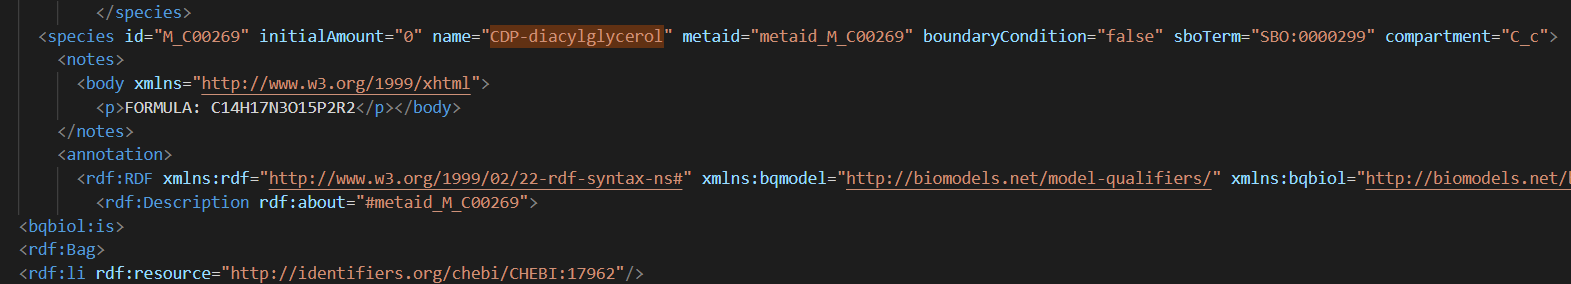
\includegraphics[width=\textwidth]{imagens/generica.png}
    \caption{Generic representation highlighted.} \label{fig2}
\end{figure}

Accordingly, biosynthetic pathways are represented in generic terms, with generic lipids as reactants and products.
Based on this, we cannot access the exact lipids used in an hypothetic biosynthetic network.
Besides that, an abstract representation is linked to the loss of specificity of individual reactions. 
The use of a generic representation will impose the utilization of many lipids in the reactions, and does not allow the transformation of a generic compound into a well defined one \cite{Aung2013}.


Interestingly, we can still see the presence of cross-references to databases with the structure of these macromolecules. However, the same structure represent a multitude of structurally defined lipids of the class under representation. In these models, the name of the lipids is defined as the name of the class under representation, which, in most cases, only includes the name of the backbone.

\subsection{Structurally defined representation in GSM models}
Contrary to the generic representation, GSM models do not usually include structurally defined lipids \cite{Schutzhold}.
In those that include, the lipid name includes both the side chains and the backbone. The side chains' name is defined by the number of carbons followed by the number and the location of double bonds as well as their stereochemistry fig3.

\begin{figure}
    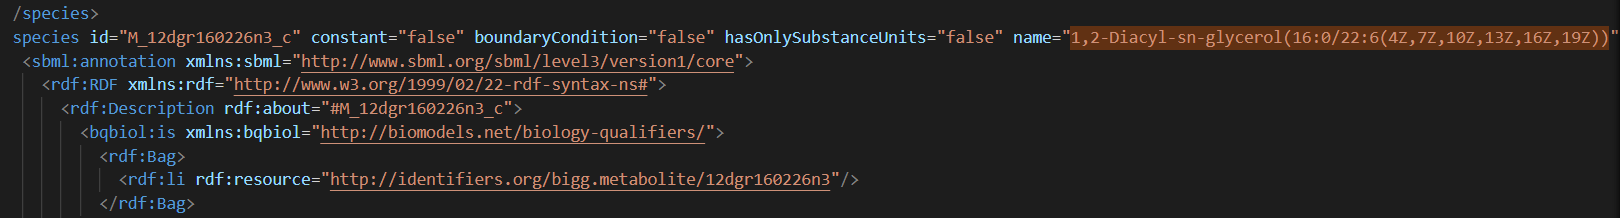
\includegraphics[width=\textwidth]{imagens/defenido.png}
    \caption{Defined representation highlighted.} \label{fig3}
\end{figure}

These approaches allow the generation of individual reactions with structurally defined lipids, in contrast with generic representations \cite{Aung2013}.
GSM models with defined lipids are more reliable, allowing the improvement of the flexibility, accuracy, and level of detail of these models. On the other hand, the inclusion of structurally defined versions of lipids can significantly increase the number of reactions in the model, which can be a drawback for some users.
Besides that, we can witness a lack of cross-references to \textit{de facto} lipid databases, which is not ideal for lipid structural confirmation, integration and interpretability.

\subsection{Lack in lipid annotation in GSM models}
 
GSM models with lipidic generic representation have few annotations to metabolites, and contrary defined ones have almost no annotation to the structure, only to the metabolites.
All things considered, the use of lipidic generic representation is not appropriate in models aiming lipid production optimization. 
But defined representation is lacking in structural annotation as well.

\begin{figure}
    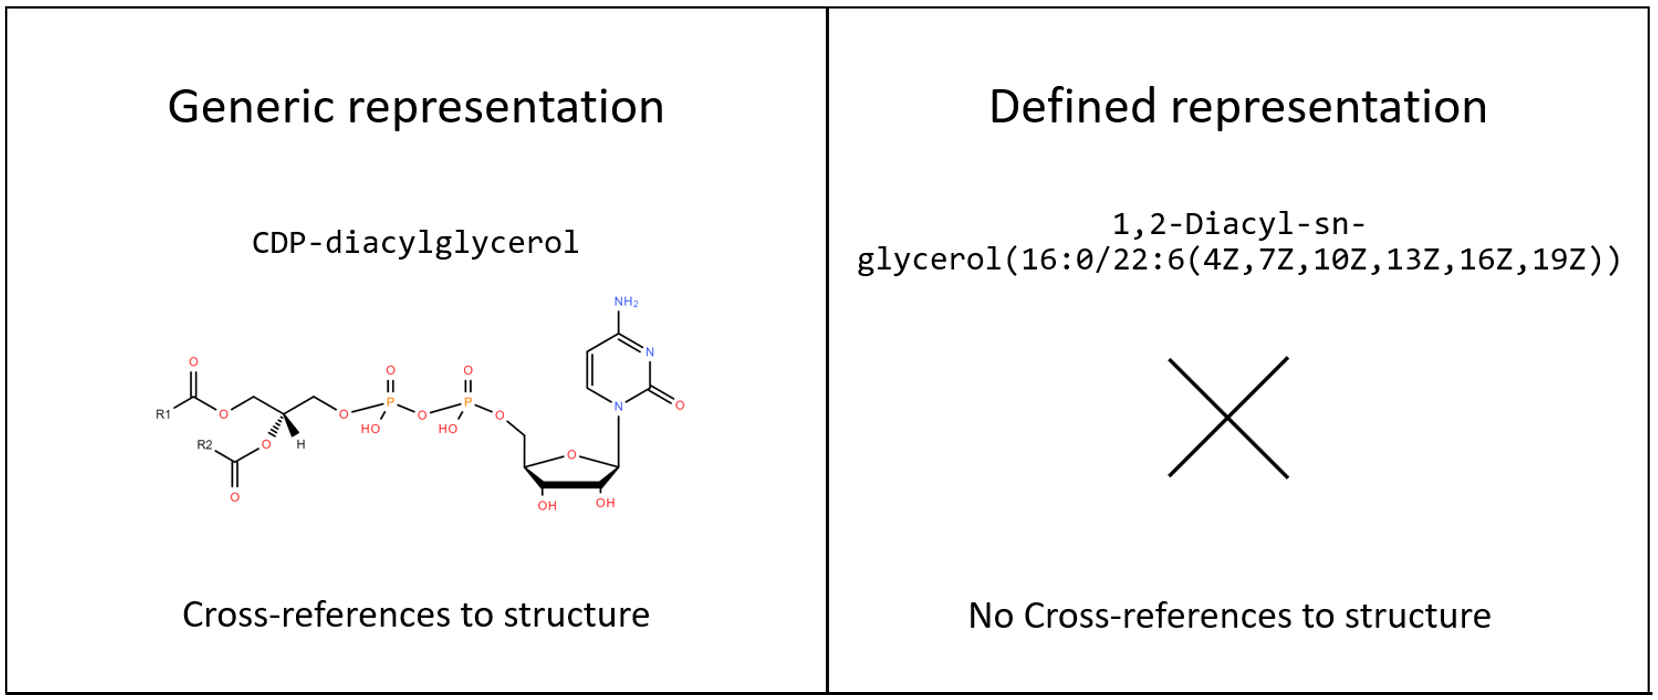
\includegraphics[width=\textwidth]{imagens/comparação.png}
    \caption{Comparation between the representations aborded above.}
\end{figure}

A possible aproche to fill this gap would be the integration of structural information in models. 
It would be achieved by the integration of synonyms and abbreviations, extracted from \textit{de facto} databases, as a link to the structural information.

ETL is a integration data tool, that allows the gathering, processing and integration of data, see Fig.\ref{fig4}. 
This is extremely usefull in data cleaning and organization providing the bases to data analytics and machine learning aproaches. 
Based on this, ETL pipelines could make more easier the integration of structural information in our database.

\begin{figure}
    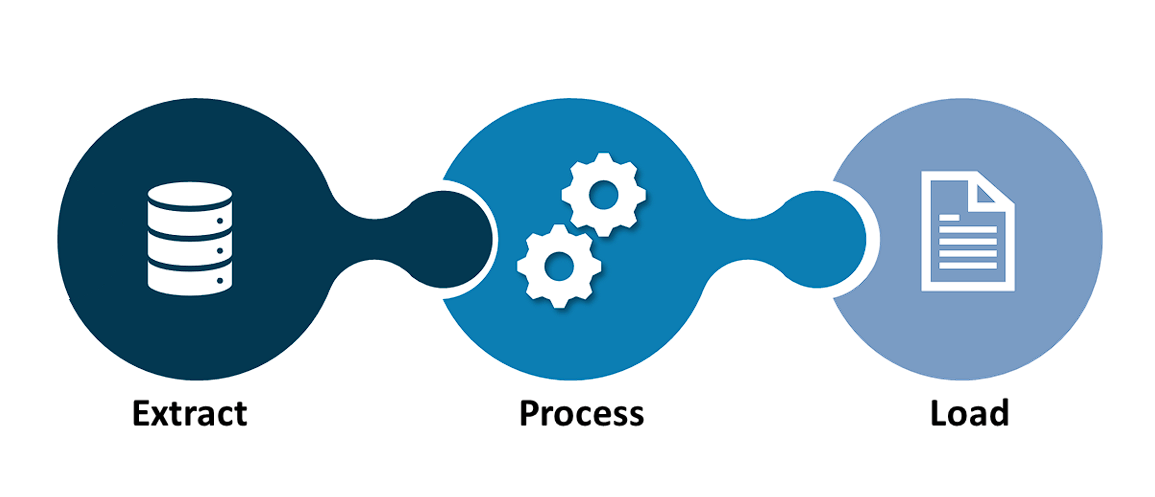
\includegraphics[width=\textwidth]{imagens/ETL.png}
    \caption{Escheme of the process done with ETL pipeline.
    First the ETL tool extracte data from multiple databases
    then processes all that data
    and finally integrates the data in our database.} \label{fig4}    
\end{figure}

Anotação de modelos:
    - match direto
    - decomposição do nome em dois (backbone e side chain) - queries à base de dados



\bibliographystyle{ieeetr}
\bibliography{referencias.bib}
\end{document}